\documentclass[12pt,a4]{article}

\newenvironment{proof}{\paragraph{Proof:}}{\hfill$\square$}

\newcommand{\handoutdate}{Thursday, 2019-09-26}
\newcommand{\firstduedate}{Monday, 2019-09-30}
\newcommand{\finalduedate}{Thursday, 2019-10-10}






\usepackage{graphicx,amsmath,amssymb,amsthm, boxedminipage}



\usepackage{algorithm}
\usepackage{algpseudocode}


\newtheorem{theorem}{Theorem}%[section]
\newtheorem{proposition}[theorem]{Proposition}
\newtheorem{lemma}[theorem]{Lemma}
\newtheorem{corollary}[theorem]{Corollary}
\newtheorem{definition}[theorem]{Definition}



\newcommand{\scalar}[2]{\ensuremath{\langle #1, #2\rangle}}
\newcommand{\floor}[1]{\left\lfloor #1 \right\rfloor}
\newcommand{\ceil}[1]{\left\lceil #1 \right\rceil}
\newcommand{\norm}[1]{\|#1\|}
\newcommand{\pfrac}[2]{\left(\frac{#1}{#2}\right)}
\newcommand{\nth}[1]{#1\textsuperscript{th}}

% \newcommand{\nth}[1]{#1\textsuperscript{th}}
\newcommand{\E}{\mathop{\mathbb{E\/}}}
\newcommand{\N}{\mathbb{N}}

\newcommand{\R}{\mathbb{R}}

\newtheorem{exercise}[theorem]{Exercise}
\newtheorem{exerciseD}[theorem]{*Exercise}
\newtheorem{exerciseDD}[theorem]{**Exercise}

\let\oldexercise\exercise
\renewcommand{\exercise}{\oldexercise\normalfont}

\let\oldexerciseD\exerciseD
\renewcommand{\exerciseD}{\oldexerciseD\normalfont}

\let\oldexerciseDD\exerciseDD
\renewcommand{\exerciseDD}{\oldexerciseDD\normalfont}


 
\begin{document}

\date{}

\title{CS 217 -- Algorithm Design and Analysis \\ 
  \vspace{3mm}
{\large	Shanghai Jiaotong University, Fall 2019\\
}
}
\maketitle

\noindent
Handed out on \handoutdate{}\\
First submission and questions due on \firstduedate{}\\
You will receive feedback from the TA.\\
Final submission due on \finalduedate{}




\setcounter{section}{2}

\section{Minimum Spanning Trees}

Throughout this assignment, let $G$ be a weighted graph, i.e., $G=(V,E,w)$ 
with $w: E \rightarrow \R^+$.
For $c \in \R$ and a weighted graph $G = (V,E,w)$, let
  $G_c := (V, \{e \in E \ | \ w(e) \leq c\})$. That is, $G_c$ is the
  subgraph of $G$ consisting of all edges of weight at most $c$.


\begin{exercise}
  Let $T$ be a minimum spanning tree of $G$, and let $c \in \R$.  Show that
  $T_c$ and $G_c$ have exactly the same connected components.  (That
  is, two vertices $u,v \in V$ are connected in $T_c$ if and only if
  they are connected in $G_c$).
  You are encouraged to draw pictures to illustrate your proof!
\end{exercise}
\begin{proof}
		In other words, we need to prove the following statements are equivalent
		, given $v_1,v_2\in V$
		\[
				\exists \text{ path } e_1,\ldots,e_{n} \in E, 
				\text{ the path connects } v_1,v_2 , \text{and } w\left( e_i \right) 
				\le  c\quad (*)
		.\] 
		and 
		\[
				\exists \text{ path } e_1,\ldots,e_{n} \in E\left( T \right) , 
				\text{ the path connects } v_1,v_2 , \text{and } w\left( e_i \right) 
				\le  c \quad  (**)
		.\] 
		Notice that $(**)\implies(*)$ is obvious. We only need to prove 
		$(*) \implies (**)$. The path connects $v_1,v_2$ in
		$T$ is unique, otherwise there are cycles.

		Let the unique path connects $v_1=u_1,\ldots,u_{t}=v_2$. 
		And assume $\exists j, 1\le j < t$ such that 
		\[
				w\left( e(u_j,u_{j+1}) \right) > c
		.\] 
		we remove the edge $e\left( u_j,u_{j+1} \right) $ from $T$, and get 2 
		sets of vertices $A,B$. $A,B$ are connected respectively. We prove
		that $\exists e \in E$ that connects $A,B$ plus  $w\left( e \right) \le c$. 
		This is obvious from $(*)$. Hence it leads that $T$ is not 
		a MST, a contradiction.
\end{proof}



\begin{exercise}
  For a weighted graph $G$, let $m_c(G) := | \{ e \in E(G) \ | \ w(e) \leq c\}|$, i.e.,
  the number of edges of weight at most $c$ (so $G_c$ has $m_c(G)$ edges).
  Let $T, T'$ be two minimum spanning trees of $G$. Show that
  $m_c(T) = m_c(T')$.
\end{exercise}
\begin{proof}
	Let the edge set of $T_c$ be 
	 \[
			 E\left( T_c \right)  = \{e_1,e_2,\ldots, e_{r}\} 
	.\]
	We know that $E\left( T_c \right) $ forms several connected componets 
	$A_1,A_2,\ldots,A_{t}\subset V$. And from the last exercise we know that 
	$A_1,A_2,\ldots,A_{t}$ are also connected componets in $T'$. 
	And we can assert the connected components in $T'$ are exactly 
	these $A_{i}$, otherwise apply the conclusion from last exercise, we can 
	derive more components for $T$.
	And 
	specifically, those components must be trees. 
	Hence 
	 \[
			 m_{c}\left( T \right) = \sum_{i=1}^{t} \left( \lvert A_{i} \rvert -1
			 \right)  = m_{c}\left( T' \right) 
	.\] 
\end{proof}


\begin{exercise}
  Suppose $G$ is connected, and no two edges of $G$ have the same weight. 
  Show that $G$ has exactly one minimum spanning tree!
\end{exercise}
\begin{proof}
		Otherwise consider 2 minimum spanning tree $T_1,T_2$, let 
		\[
				E\left( T_1 \right)  = \{a_1,a_2,\ldots, a_{r}\} 
		.\] 
		in which $a_{i}< a_{i+1}$, and similarly 
		\[
				E\left( T_2 \right)  = \{ b_1,b_2,\ldots,b_{s}\} 
		.\] 
		Let $j$ be the minimum such that $a_j \neq b_{j}$. We can assert 
		$j$ exists since $T_1,T_2$ are different. 
		
		W.L.O.G	 let $a_{j} < b_{j}$, it leads that
		\[
				m_{a_{j}} \left( T_1 \right) = j \neq j - 1
				= m_{a_{j}} \left( T_2 \right) 
		.\] 
		Which contradicts with \textbf{Exercise 2}. 
\end{proof}

A {\em multigraph} is a graph that can have multiple edges, called
``parallel edges''. Without defining 
it formally, we illustrate it:
\begin{center}
  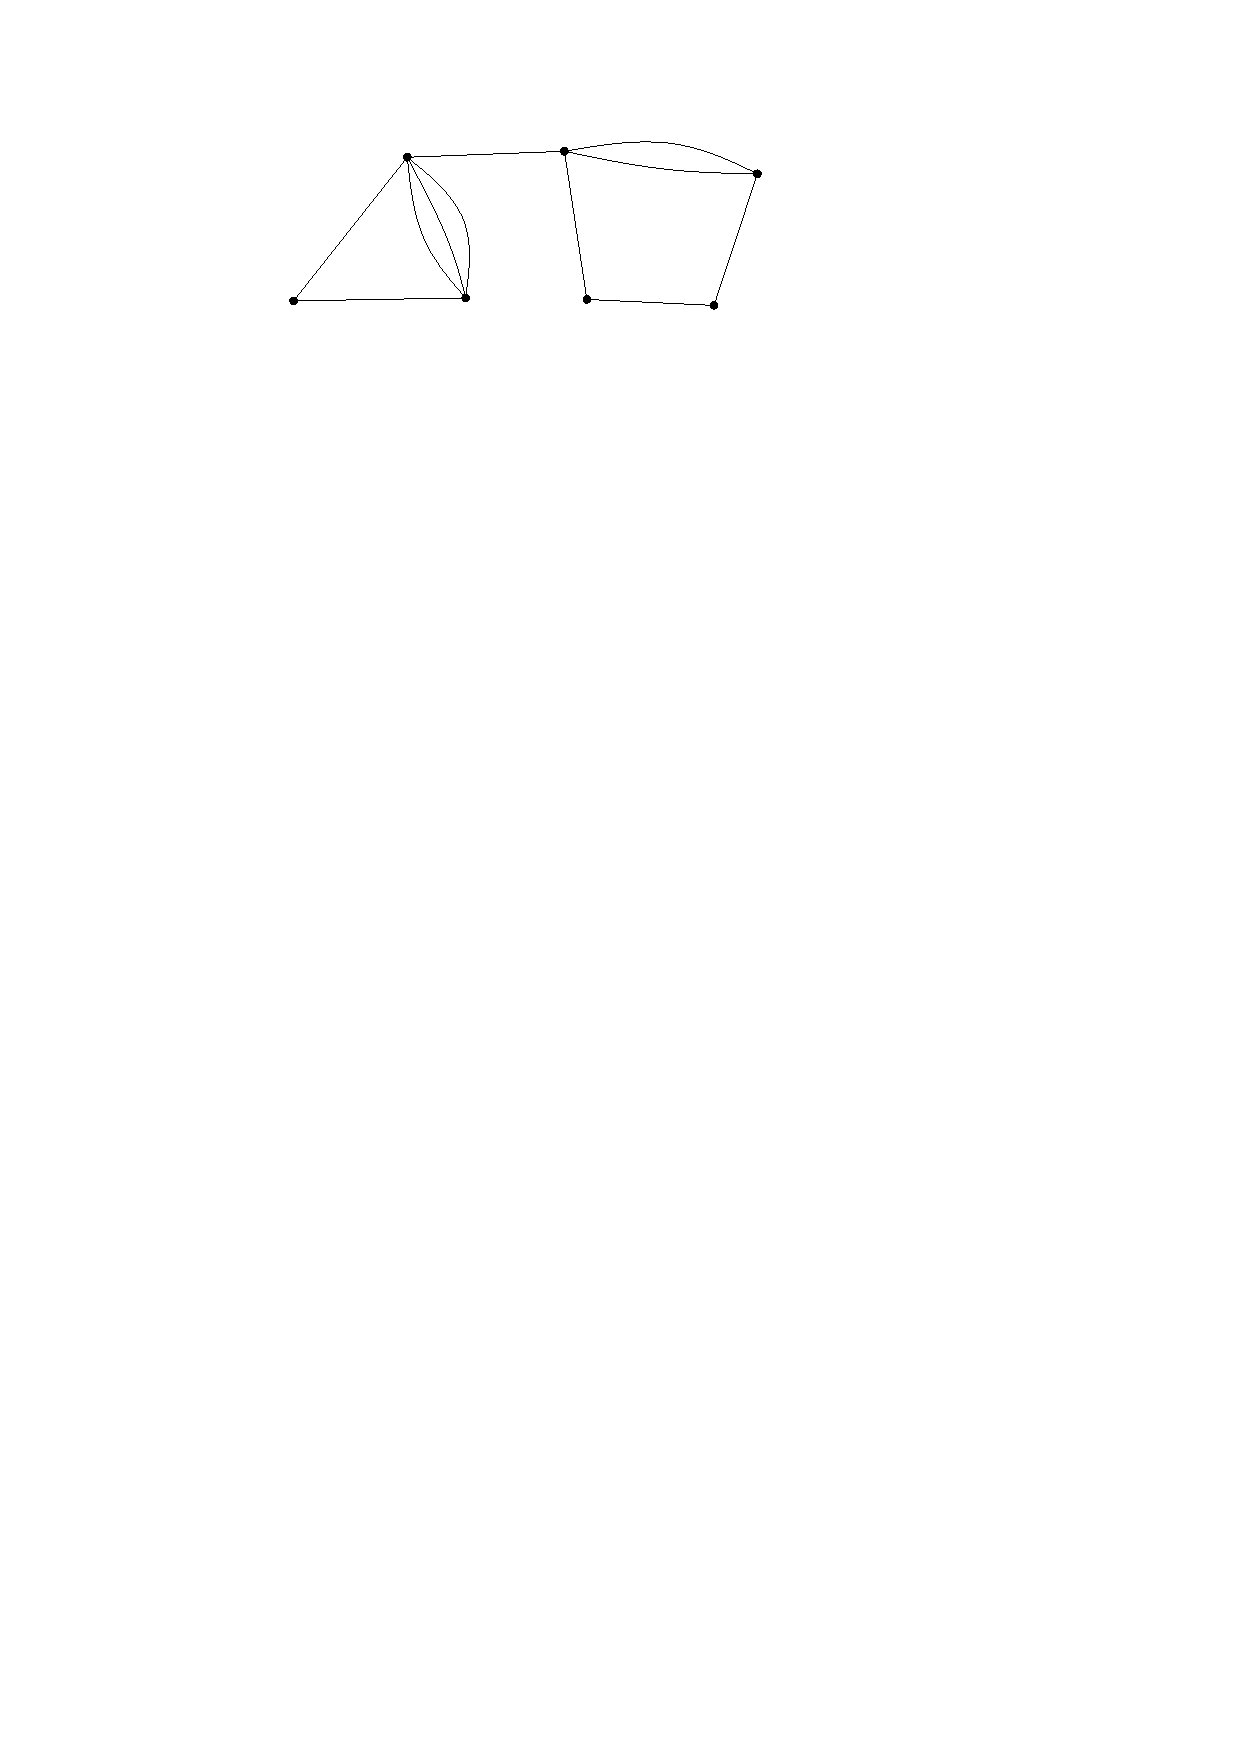
\includegraphics[width=0.6\textwidth]{figures/multigraph.pdf}\\
  A multigraph.
\end{center}
All other definitions, like connected components and spanning trees
are the same as for normal (simple) graphs. However,
when two spanning trees use different parallel edges, we consider them
different:
\begin{center}
  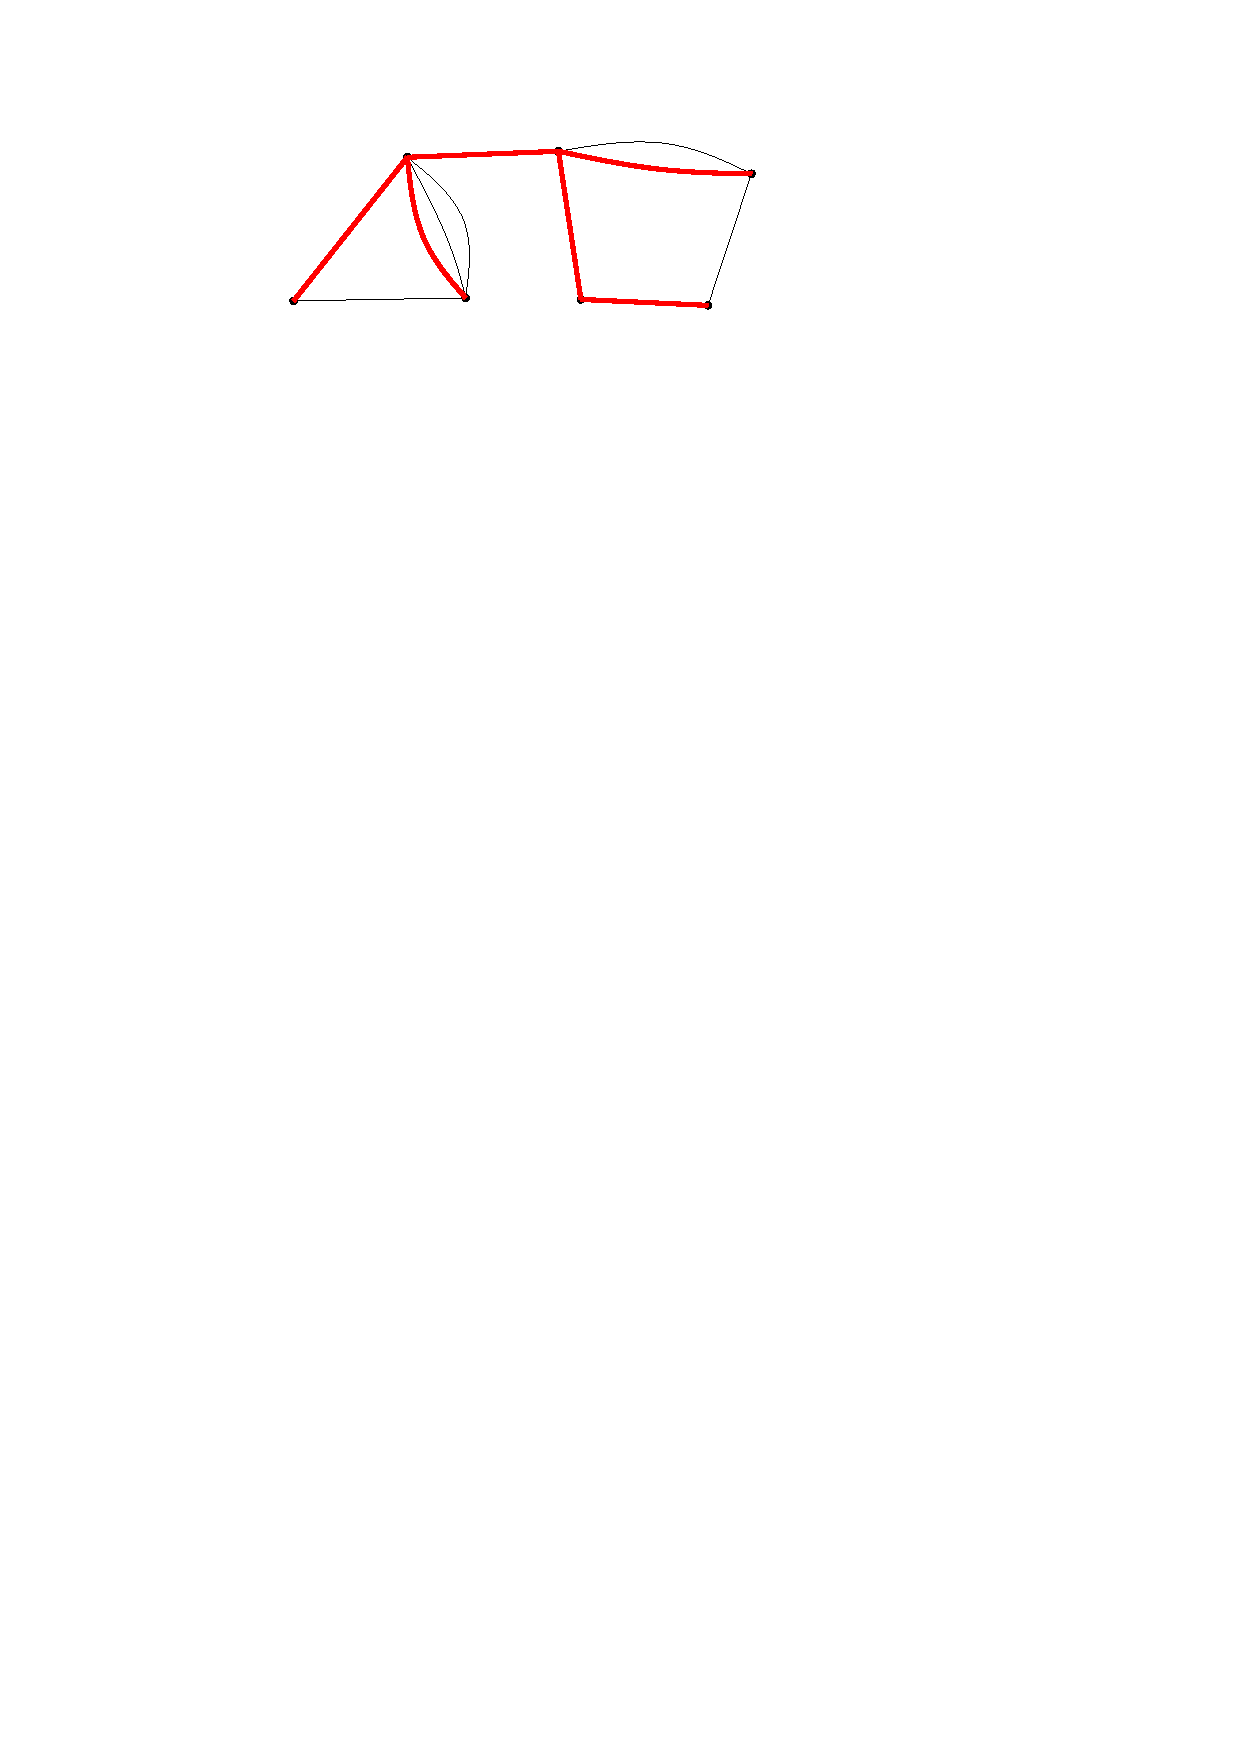
\includegraphics[width=0.4\textwidth]{figures/multigraph-forest.pdf} \hspace{2cm}
  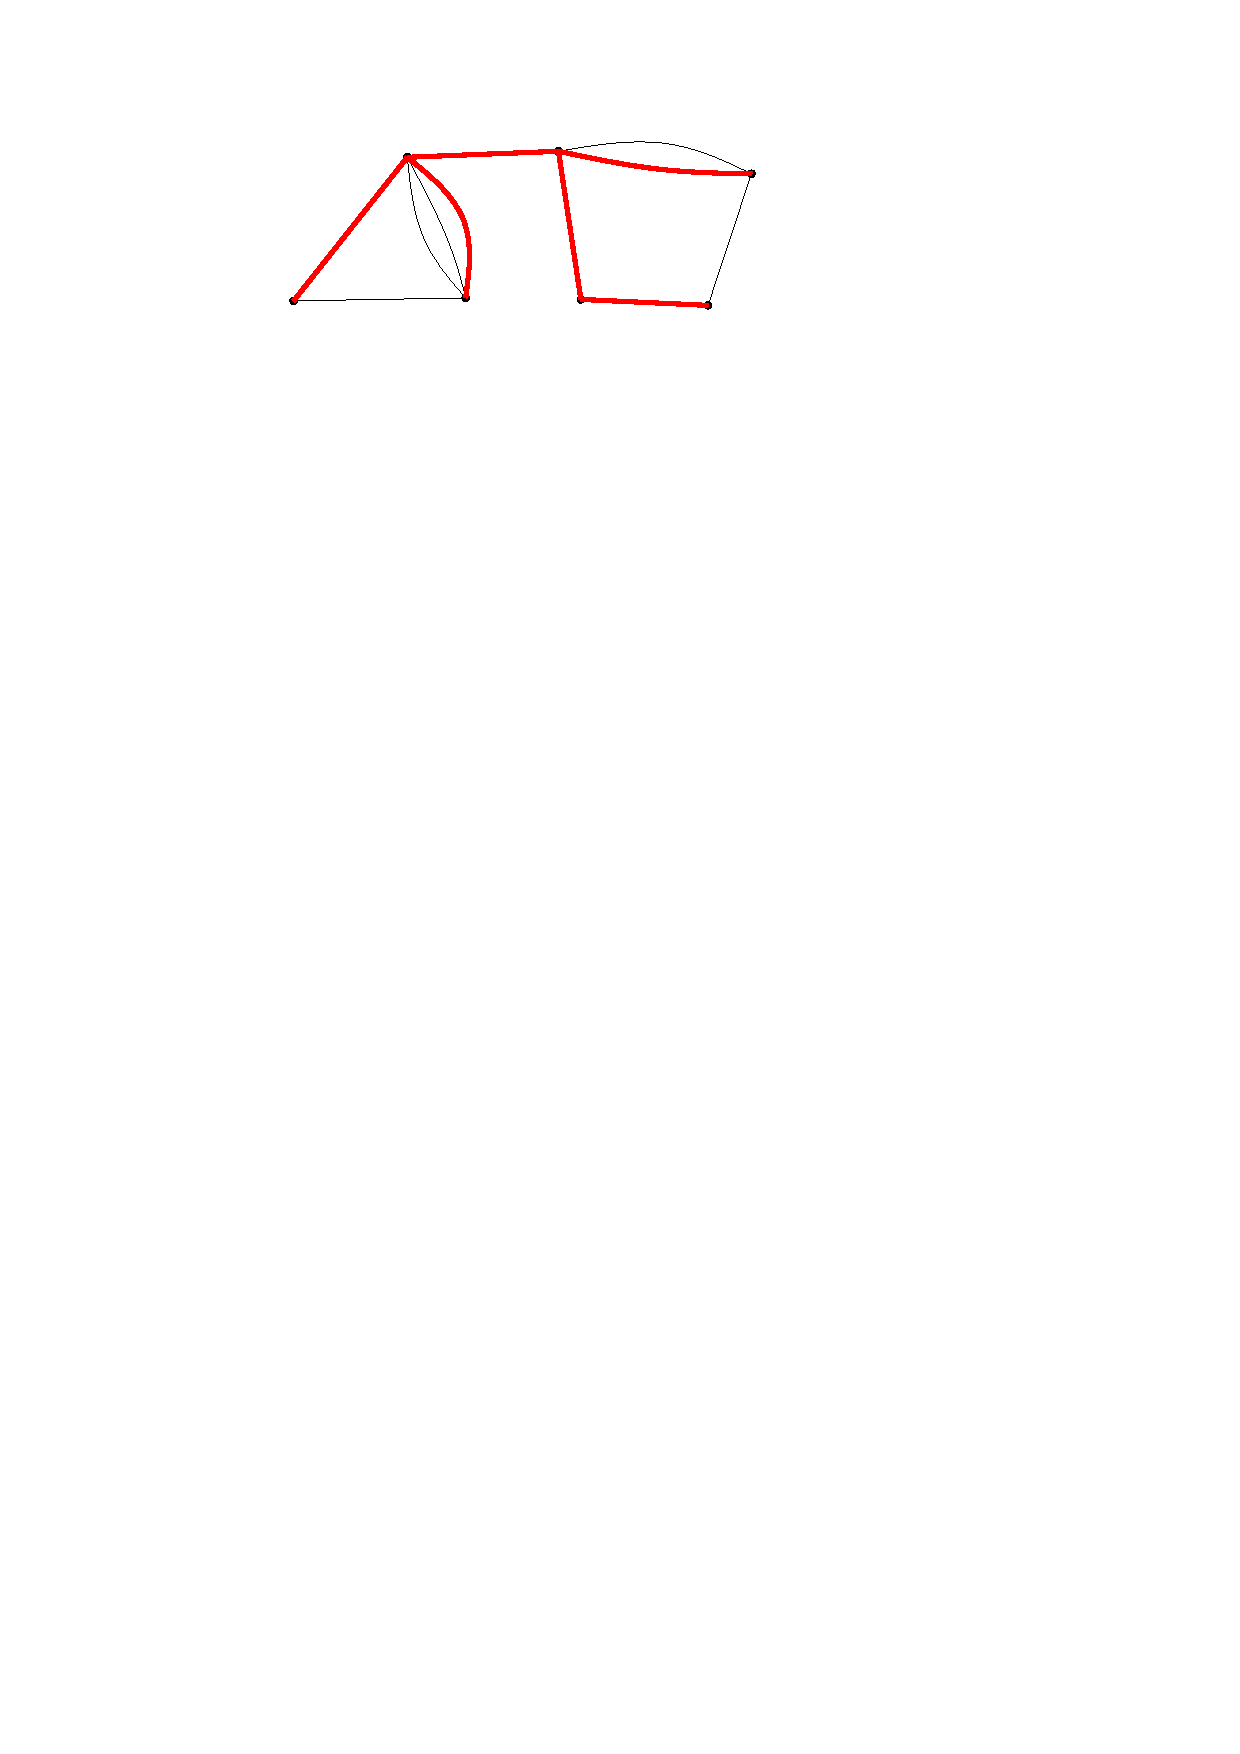
\includegraphics[width=0.4\textwidth]{figures/multigraph-forest-other.pdf} \\
  The same multigraph with two different spanning trees.
\end{center}


\begin{exercise}
  How many spanning trees does the above multigraph on 7 vertices have?
  Justify your answer!\\
\end{exercise}
\begin{proof}
		Since the edge in the middle must be chosen. We  only need to 
		consider the spanning tree in 2 subgraphs.
\end{proof}
\begin{exercise}
  Suppose you have a polynomial-time algorithm that, given a multigraph $H$,
  computes the number of spanning trees of $H$.
  Using this algorithm as a subroutine, design a polynomial-time algorithm
  that, given a weighted graph $G$, computes the number of 
  minimum spanning trees of $G$.
\end{exercise}
\begin{proof}
		
\end{proof}



\end{document}
